\chapter{Introduction}
\label{sec:Introduction}


With the advent of deep learning, a lot of applications have been needing more and more data. However, more often than not, these data contain a large amount of sensitive and personal information that restricts its use according to the legal framework in place in many countries. \\
Data is growing rapidly within companies, containing a great deal of sensitive information that can't be processed or shared without due consideration of legal ramifications. If such data could reveal the identity of someone, their personal rights would be threatened. \\
This is especially relevant in the context of HR tickets, which can contain not only personal information but also special categories of personal data, which require extra protection according to GDPR. \\


\section{GDPR}\todo{please add references to GDPR}
The General Data Protection Regulation\cite{european_commission_regulation_2016} is a privacy regulation that regulates the processing of personal data \textit{"wholly or partly by automated means and to the processing other than by automated means"}. The regulation applies to all citizens of the EU and to all data subjects in the EU, whether the processing is carried out inside or outside the EU. \\
Personal data are defined as \textit{"any information relating to an identified or identifiable natural person"}. The regulation states that \textit{"an identifiable natural person is one who can be identified, directly or indirectly, in particular by reference to an identifier such as a name, an identification number, location data, an online identifier or to one or more factors specific to the physical, physiological, genetic, mental, economic, cultural or social identity of that natural person"}. The natural person can be identified both by direct identifiers and quasi-identifiers. The direct identifiers are information that directly identify the person, such as the telephone number, social security number\dots, while the quasi-identifiers are information that alone cannot identify a person, but if they are combined with other quasi-identifiers can affect a person's privacy. For example, the job title could be not enough to identify a person, but combined with his/her company and his/her nationality it could be. \\
Moreover, the GDPR treats some categories of personal data more carefully. These categories are called 'special categories' and include racial or ethnic origin, political opinions, religious or philosophical beliefs, trade union membership, genetic data, biometric data, data concerning health or data concerning a natural person's sex life or sexual orientation.\\
The special categories of personal data cannot be generally processed, with some exceptions, including \textit{"the data subject has given explicit consent to the processing of those personal data for one or more specified purposes"}.\\

\section{Synthetic data}
Synthetic data is artificial data that is generated from real data and has the same statistical distribution as the original data \todo[inline]{there are a few different definitions here, it would be good to make a little literature search, look for examle at https://arxiv.org/pdf/2011.07018.pdf (Synthetic Data – Anonymisation Groundhog Day, Stadler) for some critic review. The idea is: synth data can or cannot have differential privacy as part of the generation process. You can use synthetic data as means to provide a certain degree of anonymization, or just as test data. It might be worth elaborating on the two macro approaches here}. This means that synthetic data and original data should deliver very similar results when undergoing the same statistical analysis. \\
Synthetic data has many benefits over real data: if you create a model that generates synthetic data you can generate how many data you need, you can infer certain properties to your data ( for example it can be useful for bias and fairness research ) and, above all, synthetic data can respect the right to personal data protection. It is important to point out that it is not always guaranteed that synthetic data is privacy-preserving: it has been shown that synthetic data can leak personal information \cite{bellovin2019privacy}.\\
% There are various approaches to guarantee privacy while generating synthetic data\cite{stadler2021synthetic}, some of these are:
% \begin{itemize}
%     \item \textbf{IndHist}: The IndHist training algorithm extracts marginal frequency counts from every data attribute of the dataset and creates a synthetic dataset S through independent sampling from the learned marginals
%     \item \textbf{BayNet}: Bayesian Networks are a directed, acyclic graph, where there is one node per random variable and a conditional probability table for each node. Bayesian networks implicitly encode the probability of a record being sampled as a product of local conditional distributions
%     \item \textbf{CTGAN}: CTGAN applies mode-specific normalization of tabular data in order to make GANs better at replicating complex distributions.
%     \item \textbf{PATEGAN}: PATEGAN builds on the Private Aggregation of Teacher Ensembles (PATE) framework to achieve DP for
%     GANs
% \end{itemize}

\section{Ticket Generation}
We created a tool that can be used to create an unlimited amount of synthetic HR tickets and we published a dataset of 16000 tickets. Each ticket, other than the ticket's text, is composed of a category, sub-category and the entities of the ticket. The tickets are not created from scratch, but starting from real-world's datasets and some prompts that help the model generate the text. \\
We did a survey internal to the company to gather some real data, and we changed the ticket generation parameters in order to respect the real data with respect to different text metrics. \\
Finally, we showed different possible use cases for the dataset:
\begin{itemize}
    \item Ticket Anonymization
    \item Ticket Classification
    \item Named Entity Recognition on tickets' entities
\end{itemize}

\section{Structure of the thesis}
The thesis is divided in two main parts: the dataset generation (\autoref{sec:Method} and \autoref{fig:complete_schema_part1}) and the possible use cases of the dataset (\autoref{sec:Use_Cases} and \autoref{fig:complete_schema_part2}).\\

First, we built a taxonomy of the tickets (\autoref{sec:taxonomy}), then we listed all the datasets which we used as a starting point to get some initial data and we explained how they were processed (\autoref{sec:datasets}). After that, we described the process of the generation of the tickets (\autoref{sec:ticket_generation}), where we showed the templates (\autoref{sec:templates}), the generative model (\autoref{sec:gpt_j}) and the parameters we can tune during the generation process (\autoref{sec:parameters}). \\
Then, we did some analysis on the generation outcomes, both on the model (\autoref{sec:architecture_analysis}) and on the tickets' texts (\autoref{sec:results}). In \autoref{sec:survey} we illustrate the survey we did to gather the test dataset. \\
Lastly, in \autoref{sec:additional_experiments} we introduced some experiments we carried out but that were not included in the final version of the application.\\

In \autoref{sec:Use_Cases} we listed the three different use cases for the dataset and their results: the classification of the tickets' categories (\autoref{sec:classification}), the anonymization of the tickets with a different approach than the standard one (\autoref{sec:anonymization}) and the named entity recognition on the entities of the tickets (\autoref{sec:ner}), where we used both a classical approach (\autoref{sec:classical_ner}) and an innovative one (\autoref{sec:ner_nc}).


\begin{figure}[h] 
    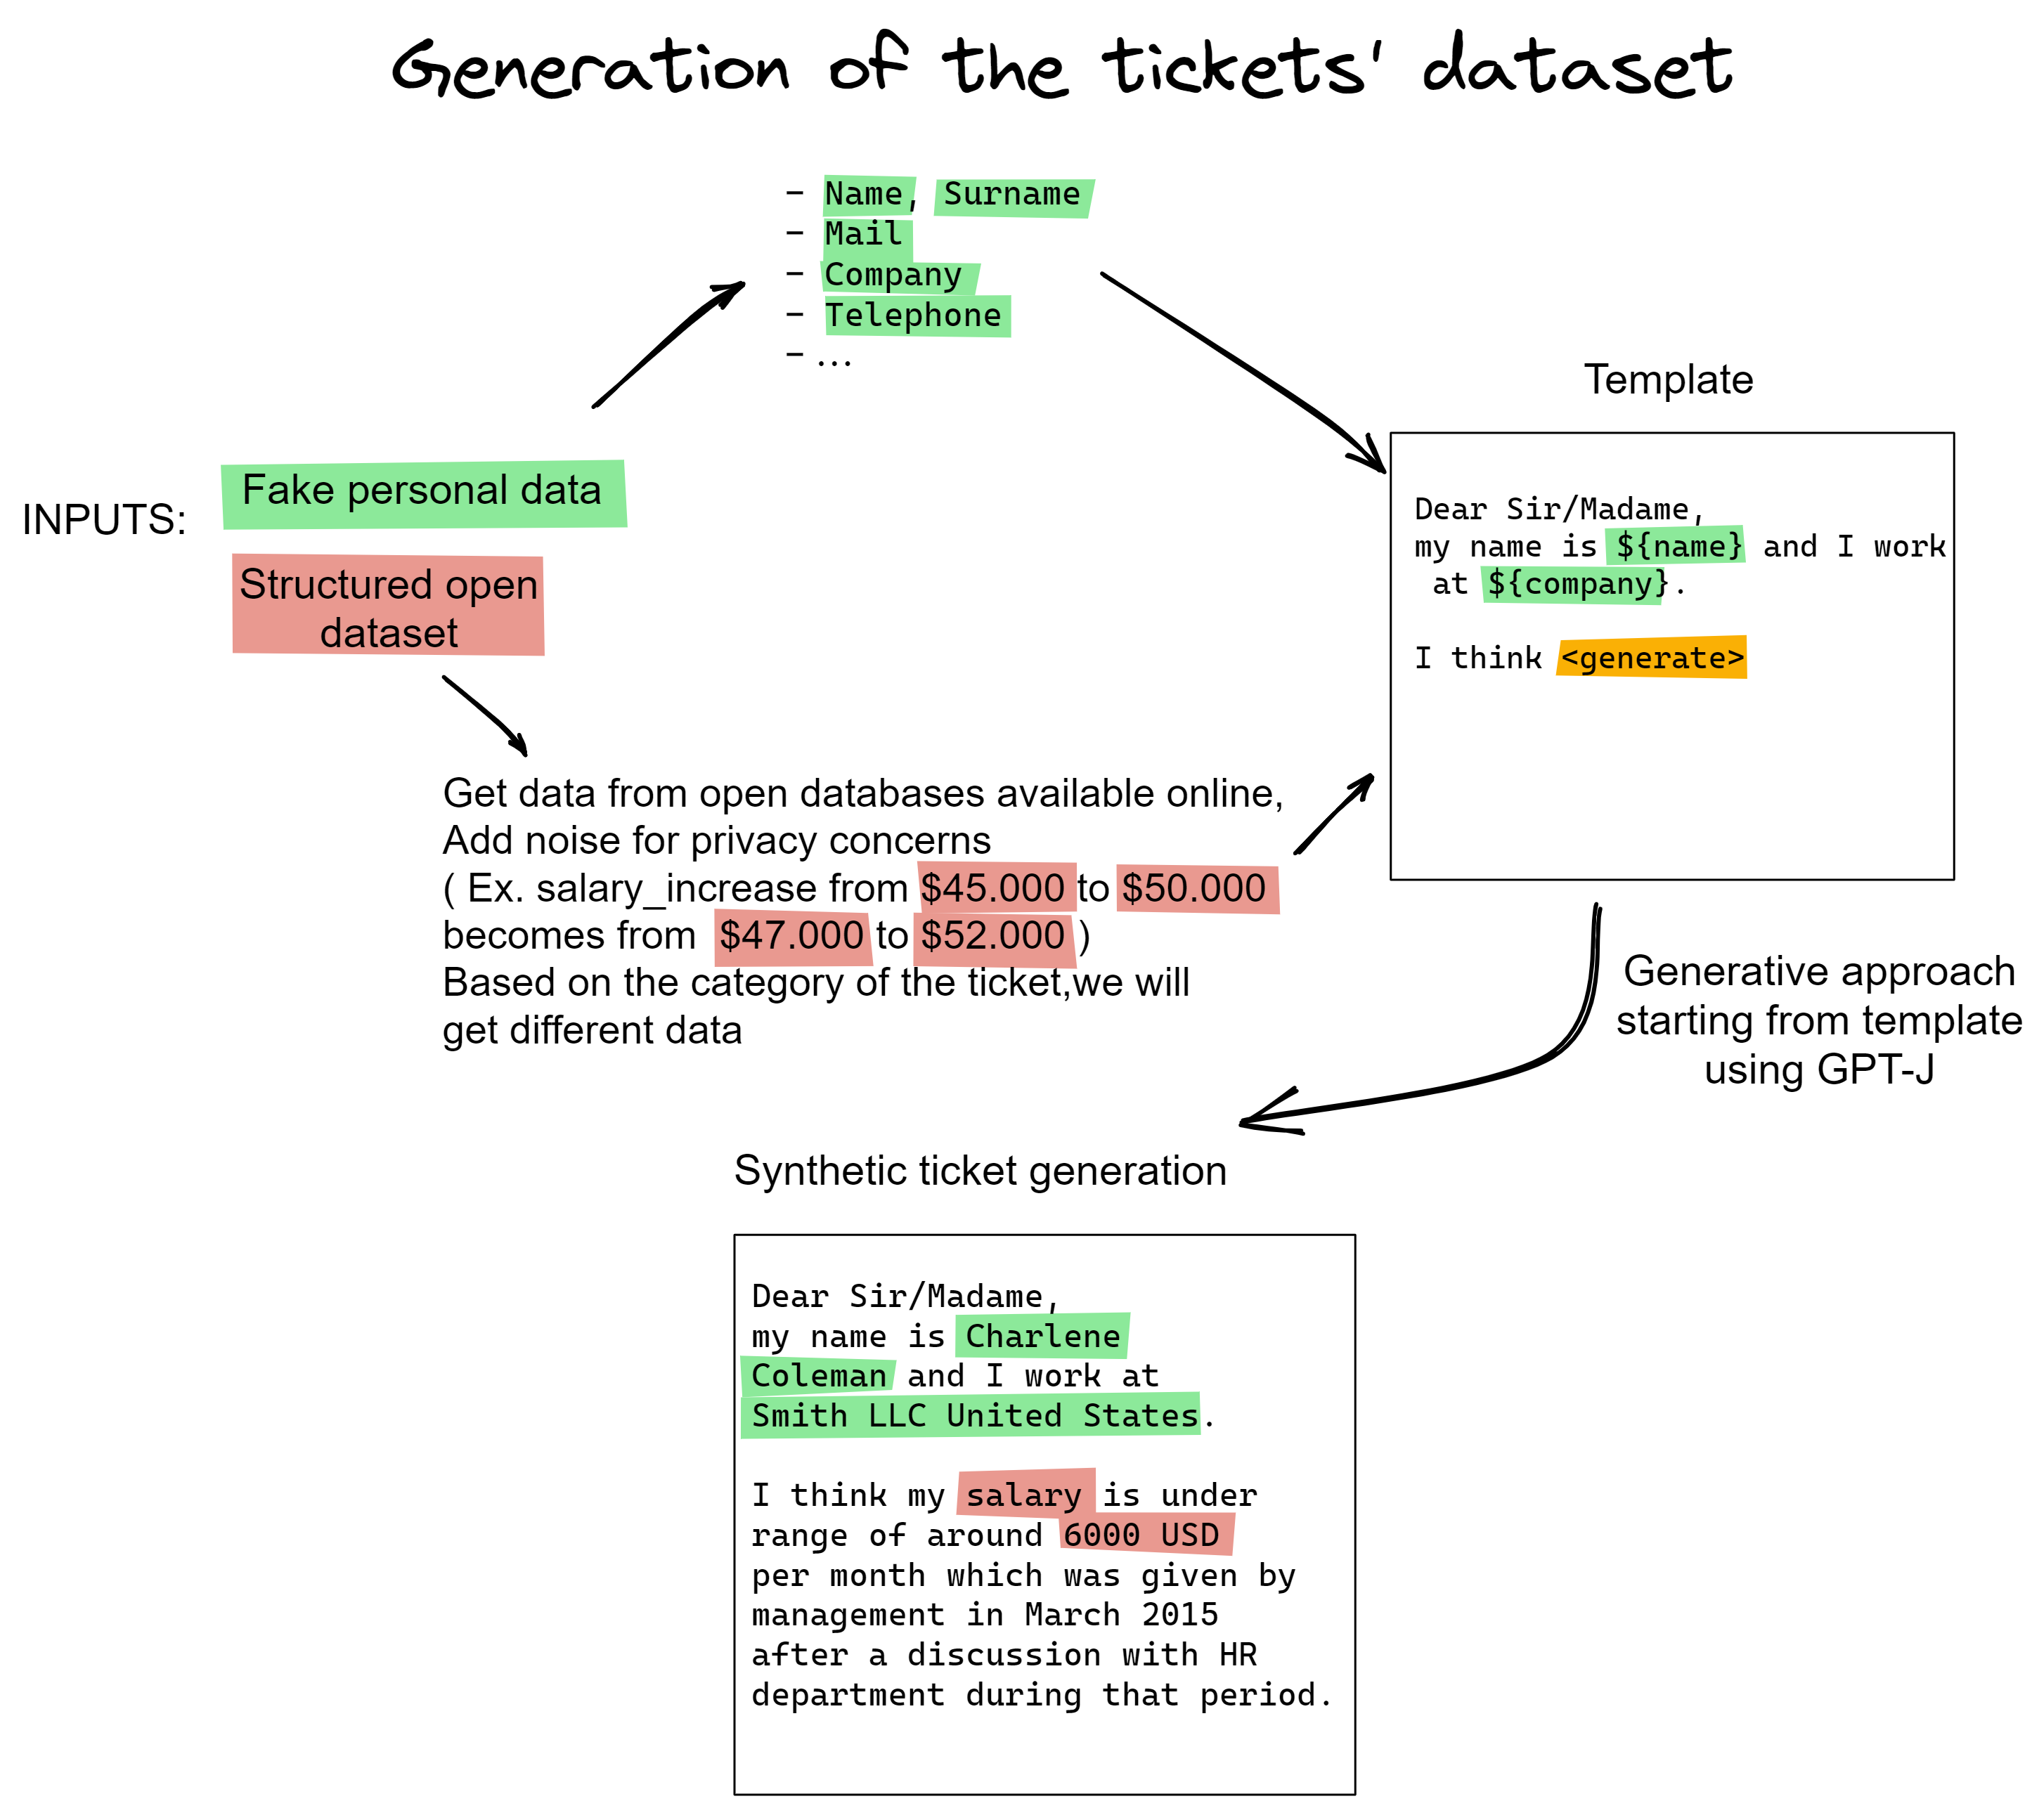
\includegraphics[width=\textwidth]{images/complete_schema_part1.png}
    \caption{Schema of the generation of the dataset}
    \label{fig:complete_schema_part1}
\end{figure}

\begin{figure}[h] 
    \centering
    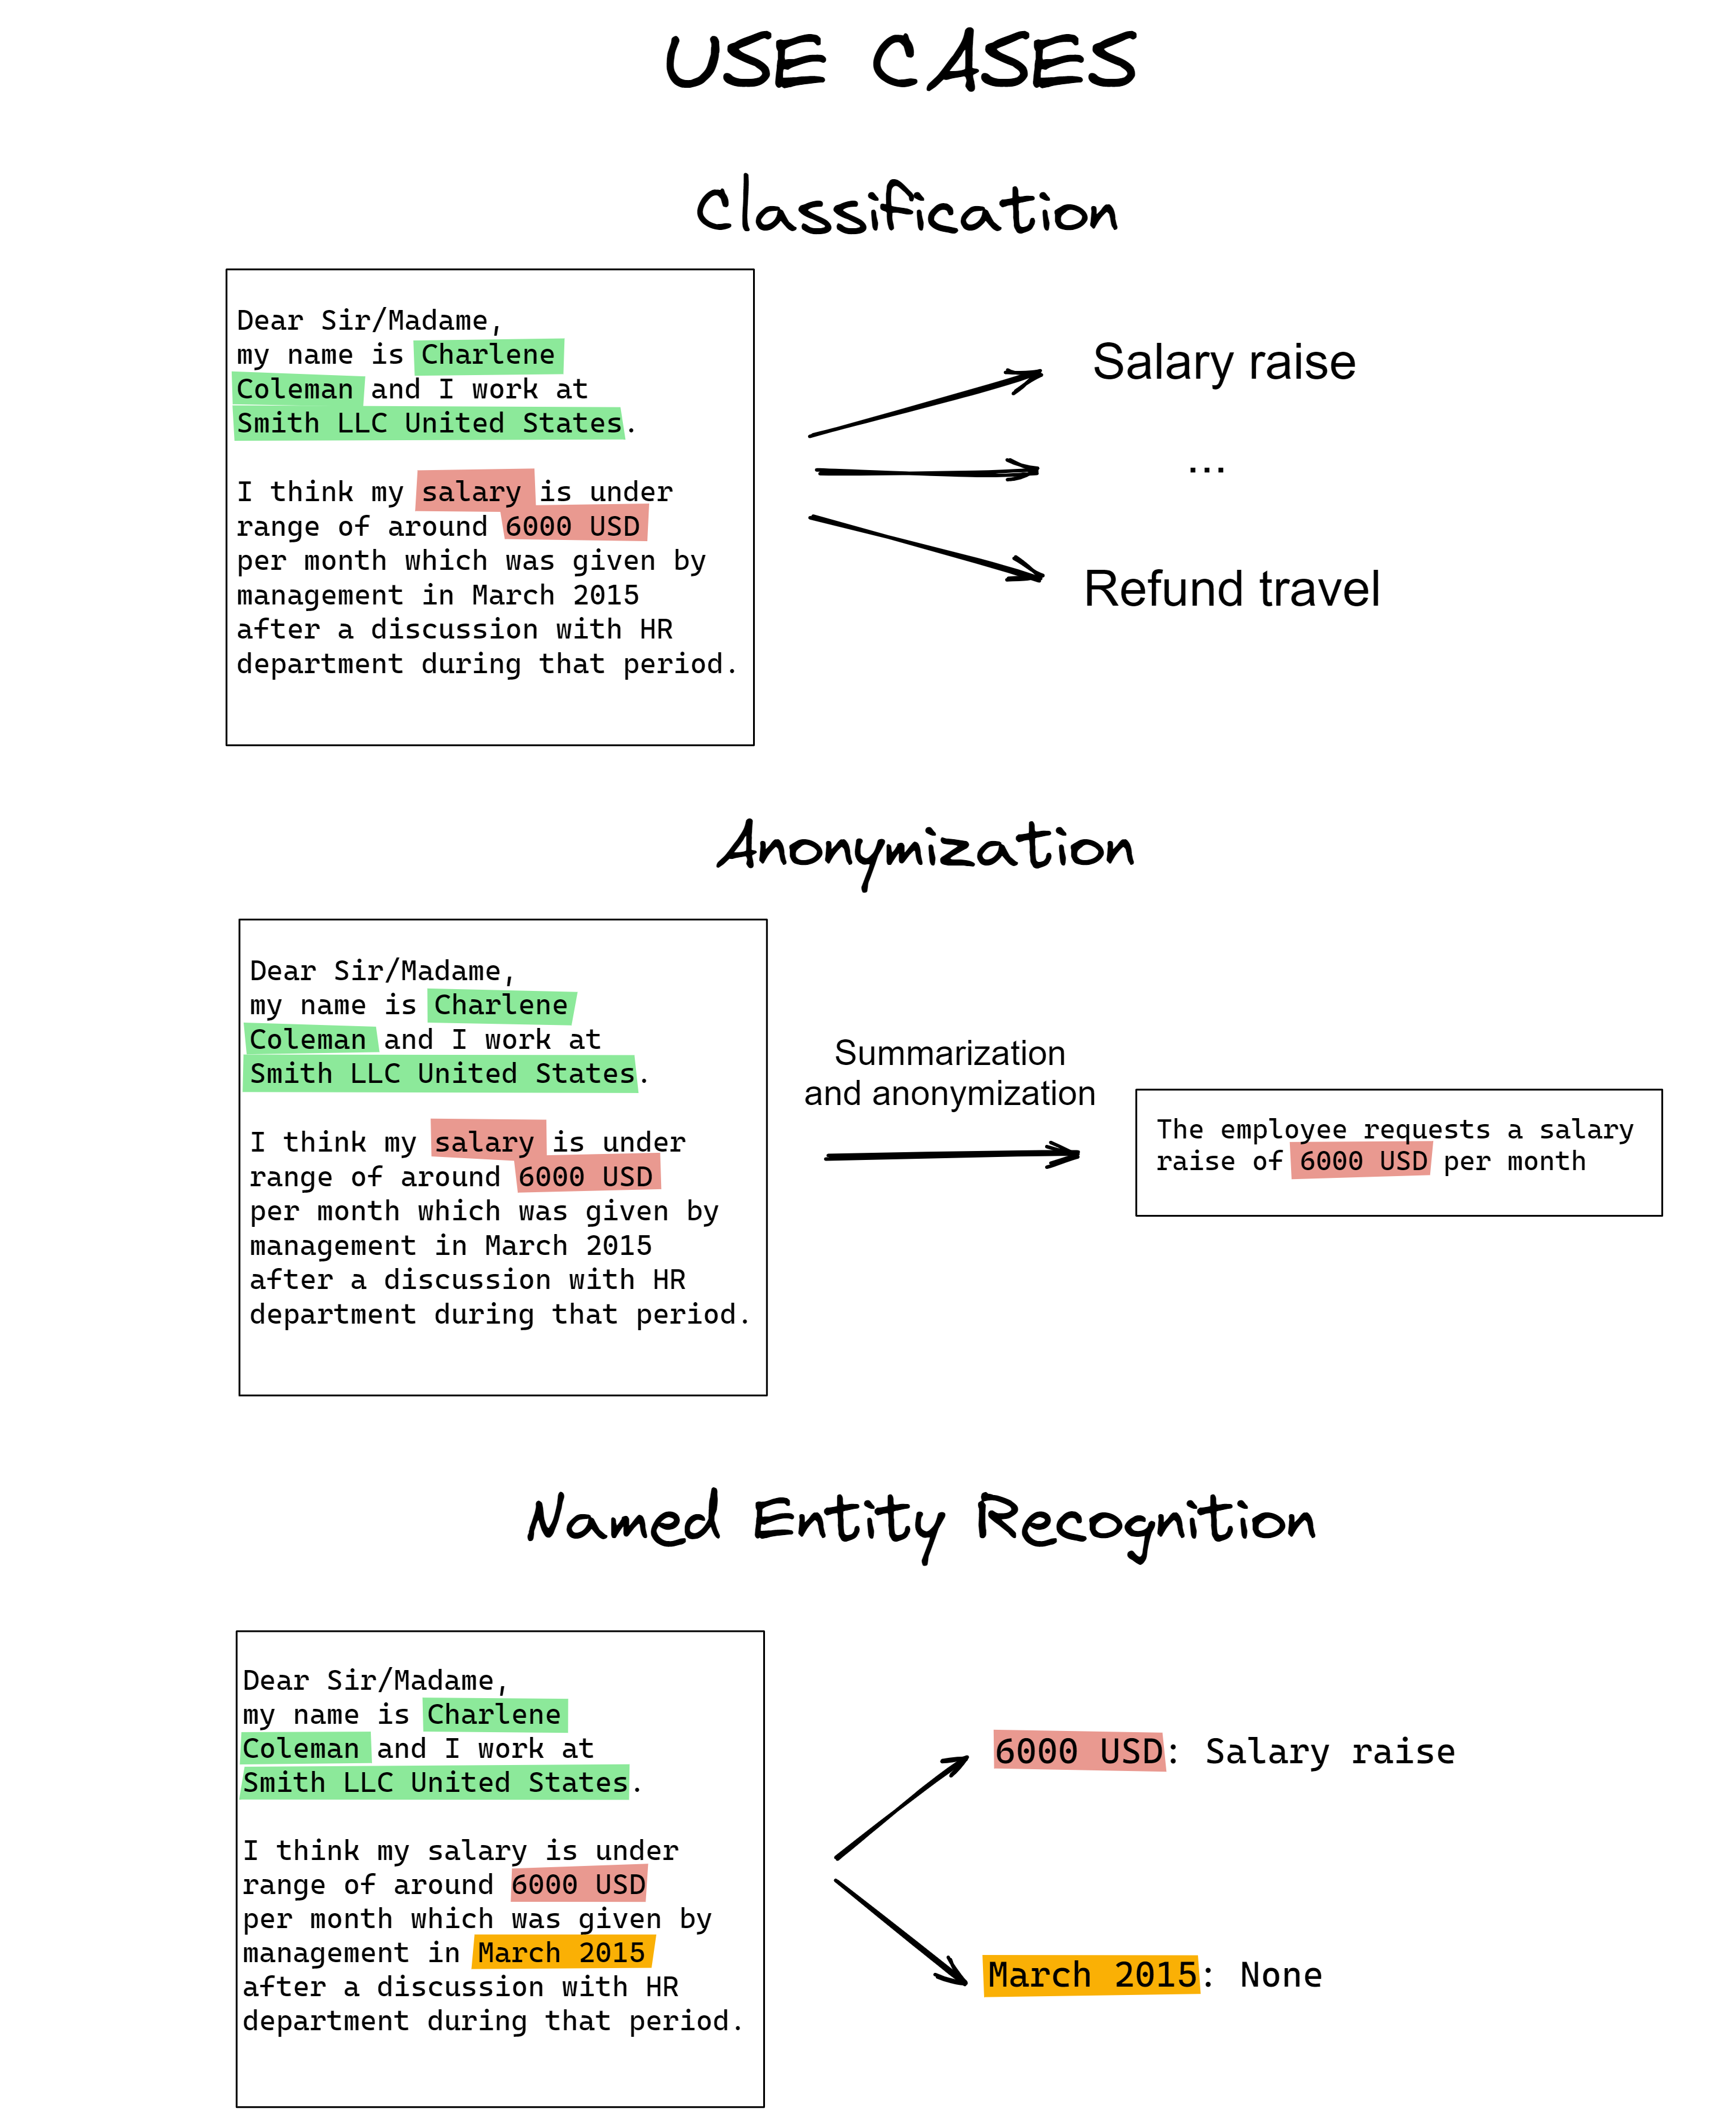
\includegraphics[width=\textwidth]{images/complete_schema_part2.png}
    \caption{Schema of the possible use cases of the dataset}
    \label{fig:complete_schema_part2}
\end{figure}    
